% Author: PokMan Ho pok.ho19@imperial.ac.uk
% Script: method.tex
% Desc: MRes thesis methods section
% Input: none
% Output: none
% Arguments: 0
% Date: Apr 2020

\documentclass[../thesis.tex]{subfiles} %% use packages & commands as this main file

\begin{document}
\section{Methodology}

\subsection{the ODE model}
The minimalist model used was composed by two players/ecological engines and three finite carbon pools (Fig.\ref{modelInWord}).  Photocells (P) and bacterial decomposers (B) were the two engines powering the interactions.  The engines themselves did not contain carbon under the model's logic and only consist of cellular biochemical reactions.  Both engines were sharing all but one different link, which is where they get carbon.  P gained carbon from the external unlimited carbon pool (i.e. $CO_2$) while B gained from the finite organic carbon (C) pool.  Both engines respired, leaked carbon and allocated the rest to its biomass carbon pool.  Also, biomass pools contained fatalities and those portions were fed into the C pool along with the leaked carbon.  At the C pool, carbon could either being ingested by B or removed from the system (artificially).  The whole system would be an independent open ecosystem if the (artificial) removal flux tuned to zero.

\begin{figure}[H]
    \centering
    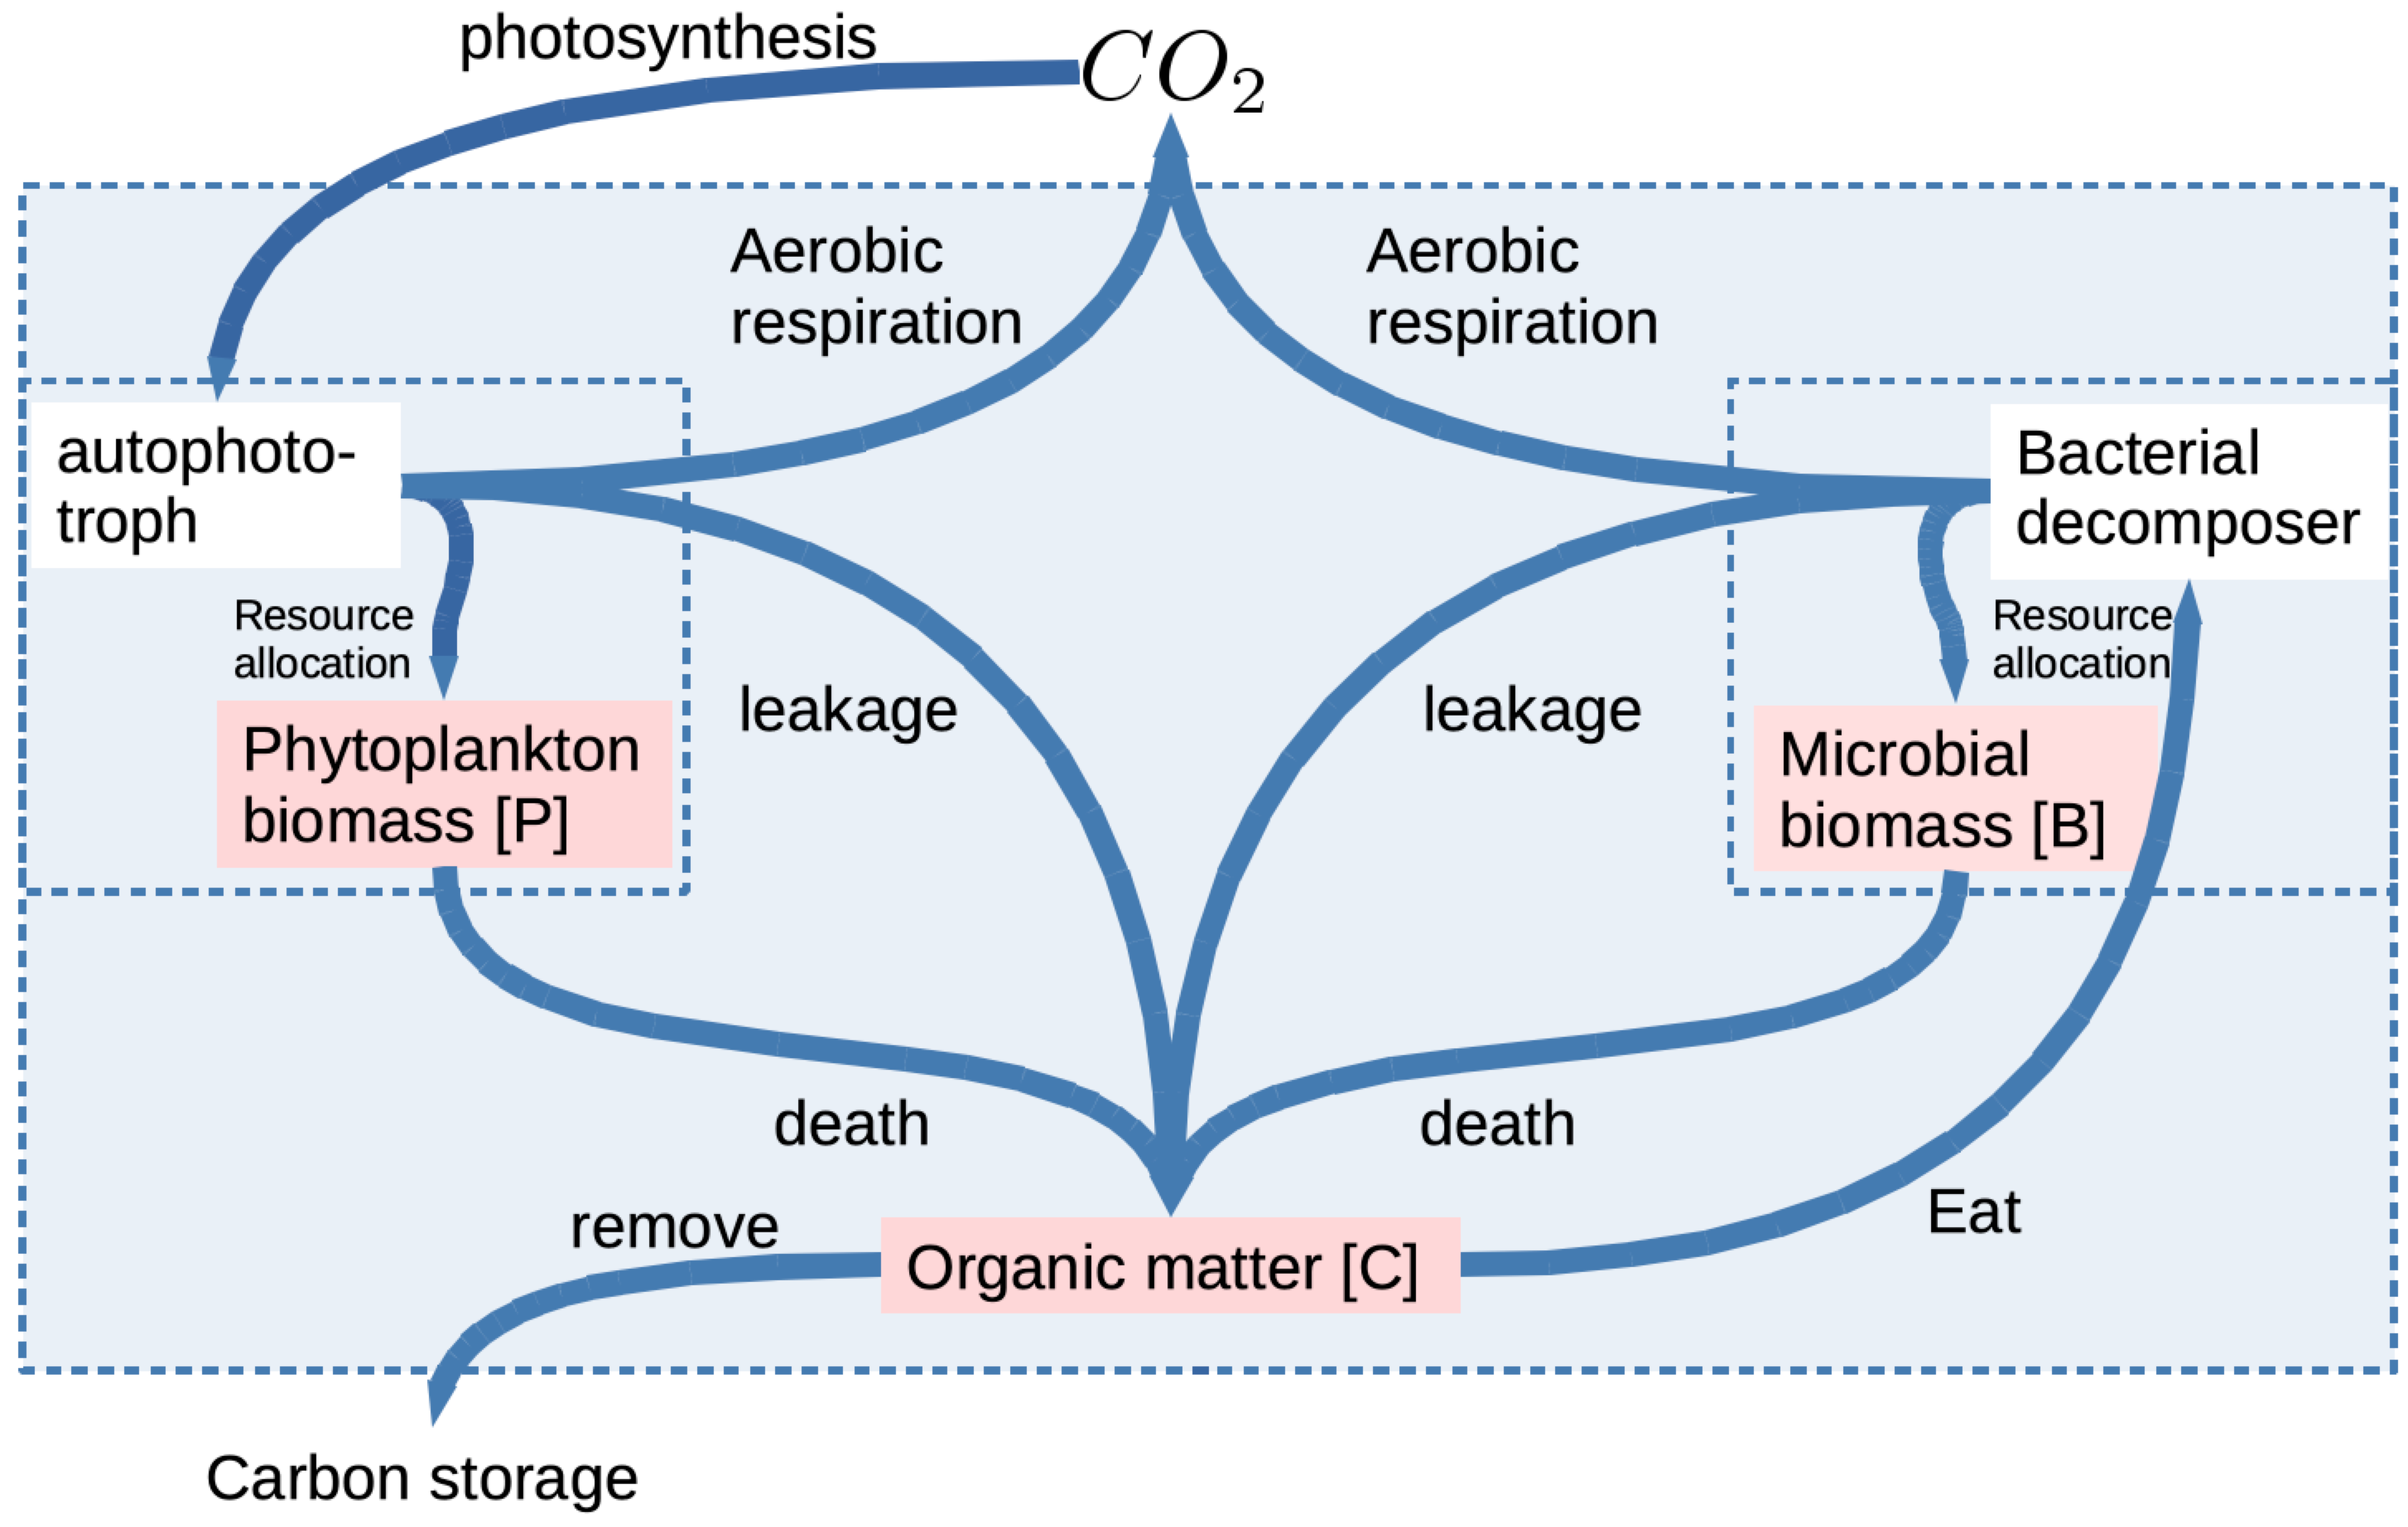
\includegraphics[width=.8\linewidth]{code/thesisSec/model.png}
    \caption[Model visualization]{Classification of dominant interactions in this project.  The two players shared all interactions with respective carbon pools but one, which was the energy acquiring method.}
    \label{modelInWord}
\end{figure}

\subsection{variables in the model}
Nine parameters were used to describe the system, two sets of four biological parameters for the players P and B plus one carbon removal rate parameter.  Due to the parameter values obtained, the finest time scale of this model was set as ``day".  $\ePR$ and $\eBR$ were non-respired carbon fractions for P and B respectively.  $\eP$ and $\eB$ were carbon fractions incorporated into biomass for P and B respectively.  These two fractions were unit-less and modeled using different parameters because experimentally these numbers were measured using different methods.  $\gP$ and $\gB$ were specific growth rates for P and B with different units.  Due to the model being an open system, $\gP$ only depended on P because the interacting counterpart was assumed being unlimited.  However, a finite resource pool C had made $\gB$ depended on both the resource (i.e. C) and consumer (i.e. B) density.  In this project, since it was assumed that the environment was homogeneous, $\gB$ was logically sounded to take units rate ($t^{-1}$) and rate per unit density($m^3/(gCt)$) as equivalent.  Death rates in the model were logically different between P and B.  $\aP$ was a mechanistic death term for P based on intraspecific interference, one of the reasons leading to carrying capacity.  On a contrary, $\mB$ was a simple specific death rate for B.  Hence this model had an intrinsic assumption, which assumed the only limiting factor for P was competition (the intraspecific interference) while that for B was the carbon resource availability.  Detailed version of calculating some parameters was in the Appendix.

\begin{table}[H]
    \centering
    \caption[Algebra variables]{Table showing variables and corresponding values used in the ODE system}
    \begin{tiny}
    \csvautotabular[]{thesisSec/varTab.csv}
    \end{tiny}
    \label{varInTab}
\end{table}

\subsection{terms included in the model}

\begin{table}[H]
    \centering
    \caption[Processes in algebra terms]{Table showing processes in Fig.\ref{modelInWord} direct translation into mathematical terms}
    \csvautotabular[]{thesisSec/termTab.csv}
    \label{termInTab}
\end{table}

\subsection{the model in equations}

\begin{equation*}\left\{\begin{array}{rl}
    C'(t) &= \ePR(1-\eP)\cdot\gP\cdot P +\aP\cdot P^2 +(\eBR(1-\eB)-1)\cdot\gB\cdot C\cdot B +\mB\cdot B -xC\\
    P'(t) &= \ePR\cdot\eP\cdot\gP\cdot P -\aP\cdot P^2\\
    B'(t) &= \eBR\cdot\eB\cdot\gB\cdot C\cdot B -\mB\cdot B
\end{array}\right.\end{equation*}

\subsection{solving the model}

\subsection{temperature standardisation}

\end{document}